
\subsection{Задача № 1}
Докажем
\begin{enumerate}
    \item $1 \Rightarrow 2$. Выполнена формула $A \& \neg A$.
    \item $2 \Rightarrow 3$. Используем аксиому $4,5$, чтобы получить $\alpha$ и $\neg \alpha$ и используем принцип Взрыва, чтобы доказать $A \&\neg A$. Воз
    \item $3 \Rightarrow 4$. Используем аксиому $4,5$, получим, что для $\alpha = A$ выполнено
    \item $4 \Rightarrow 1$. Используем принцип Взрыва и получим то, что надо
\end{enumerate}

\subsection{Задача № 2}

\begin{enumerate}
    \item[a.] 2 мира $w_0, w_1$.  Связаны $w_0 \leq w_1$ 

    Для первого мира:
$$\not\Vdash A, \not \Vdash B$$
    Для второго мира:
$$\Vdash A, \not \Vdash B$$
    Покажем, что $((A \rightarrow B) \rightarrow A) \rightarrow A$ не выполнено в данной модели Крипке:

    В $w_0$ не выполнено: 
    $$A \rightarrow B$$
    При этом тогда $\Vdash (A \rightarrow B) \rightarrow A$ выполнено и в $w_0$ и $w_1$. Заметим, что тогда не может быть выполнено:
    $$((A \rightarrow B) \rightarrow A) \rightarrow A$$
    Потому что тогда $w_0 \Vdash A$, что не так
    
    \item[b.] 2 мира $w_0, w_1$. Связаны $w_0 \leq w_1$ 

    Для первого мира:
$$\not\Vdash A, \not \Vdash B$$
    Для второго мира:
$$\Vdash A, \Vdash B$$
    Покажем, что $(A \rightarrow B) \rightarrow \neg A \lor B$ не выполнено в данной модели Крипке:

    В $w_0$ и $w_1$ выполнено: 
    $$A \rightarrow B$$
    Поймем выполнено ли $\neg A \lor B$ в $w_0$:
    $$w_0 \not \Vdash B, w_0 \not \Vdash \neg A \Rightarrow w_0 \not \Vdash \neg A  \lor B$$
    Заметим, что тогда в $w_0$ не выполняется наше условие
    \pagebreak
    \item[c.] 5 миров: $w_1, \ldots w_5$. Отношение порядка задается таким графом:
    \begin{center}
         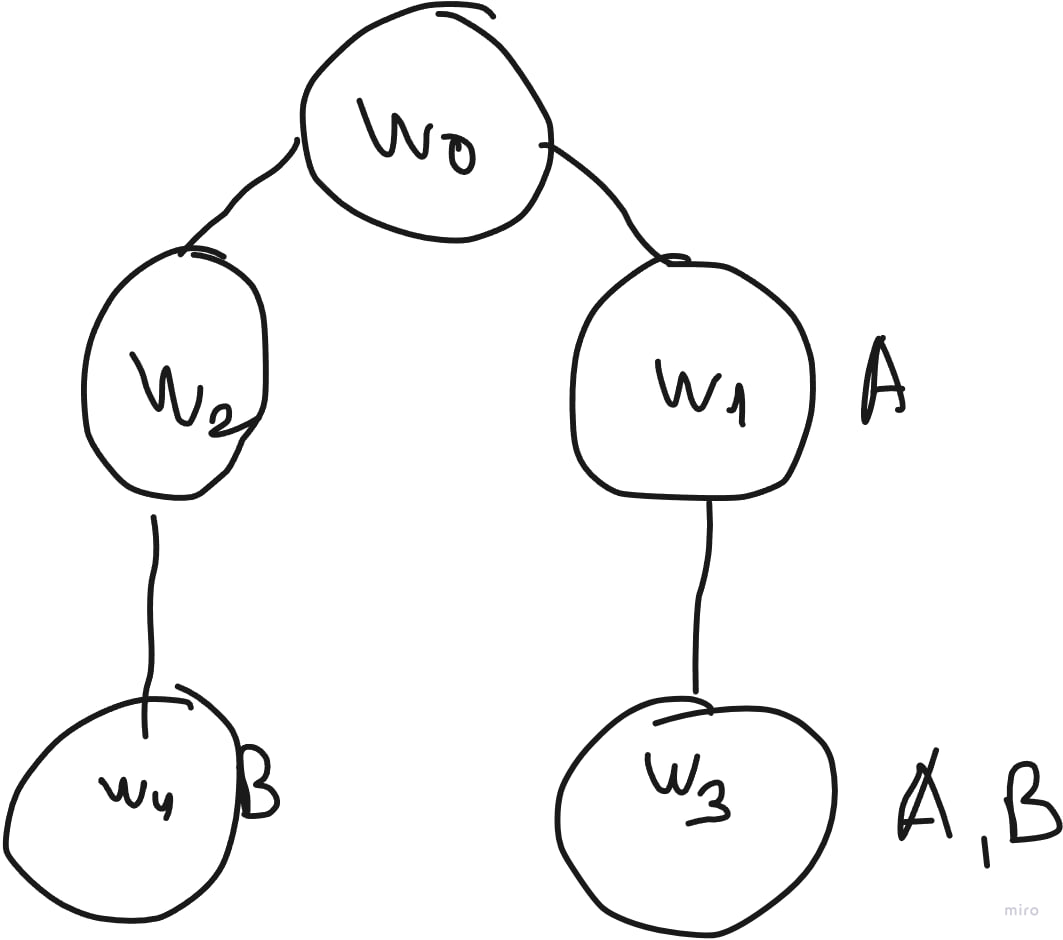
\includegraphics[width=6cm]{assets/graf.jpg}
    \end{center}
    $w_1 \Vdash A, w_4 \Vdash B, w_3 \Vdash A, w_3 \Vdash B$

    Проверим $B \lor \neg B$ для каждого мира:
    \begin{enumerate}
        \item[$w_0$] $w_0 \not\Vdash \neg B,w_0 \not \Vdash B \Rightarrow w_0 \not \Vdash B \lor \neg B $
        
        \item[$w_1$] $w_1 \not\Vdash \neg B,w_1 \not \Vdash B \Rightarrow w_1 \not \Vdash B \lor \neg B $
        
        \item[$w_2$] $w_2 \not\Vdash \neg B,w_2 \not \Vdash B \Rightarrow w_2 \not \Vdash B \lor \neg B $
        
        
        \item[$w_3$] $w_3  \Vdash B \Rightarrow w_3  \Vdash B \lor \neg B $
        
        
        \item[$w_4$] $w_4  \Vdash B \Rightarrow w_4  \Vdash B \lor \neg B $
    \end{enumerate}

    Проверим $A \rightarrow (B \lor \neg B)$ в $w_0$. Если $\Vdash A \rightarrow (B \lor \neg B)$, то в $w_0 \Vdash B \lor \neg B$, что не так. 

    Откуда в $w_0$ $\not \Vdash A \rightarrow (B \lor \neg B)$.

    Проверим $\neg A \rightarrow (B \lor \neg B)$ в $w_0$. Если $\Vdash \neg A \rightarrow (B \lor \neg B)$, то в $w_2 \Vdash B \lor \neg B$, что не так.

    Откуда в $w_0$ $\not \Vdash \neg A \rightarrow (B \lor \neg B)$.

    Отсюда очевидно, что в $w_0$ не выполнено искомое утверждение, что и надо доказать.

    
    
\end{enumerate}